\documentclass[]{article}
\usepackage[T1]{fontenc}
\usepackage{lmodern}
\usepackage{amssymb,amsmath}
\usepackage{ifxetex,ifluatex}
\usepackage{fixltx2e} % provides \textsubscript
% use upquote if available, for straight quotes in verbatim environments
\IfFileExists{upquote.sty}{\usepackage{upquote}}{}
\ifnum 0\ifxetex 1\fi\ifluatex 1\fi=0 % if pdftex
  \usepackage[utf8]{inputenc}
\else % if luatex or xelatex
  \ifxetex
    \usepackage{mathspec}
    \usepackage{xltxtra,xunicode}
  \else
    \usepackage{fontspec}
  \fi
  \defaultfontfeatures{Mapping=tex-text,Scale=MatchLowercase}
  \newcommand{\euro}{€}
\fi
% use microtype if available
\IfFileExists{microtype.sty}{\usepackage{microtype}}{}
\usepackage[margin=1in]{geometry}
\usepackage{longtable,booktabs}
\usepackage{graphicx}
% Redefine \includegraphics so that, unless explicit options are
% given, the image width will not exceed the width of the page.
% Images get their normal width if they fit onto the page, but
% are scaled down if they would overflow the margins.
\makeatletter
\def\ScaleIfNeeded{%
  \ifdim\Gin@nat@width>\linewidth
    \linewidth
  \else
    \Gin@nat@width
  \fi
}
\makeatother
\let\Oldincludegraphics\includegraphics
{%
 \catcode`\@=11\relax%
 \gdef\includegraphics{\@ifnextchar[{\Oldincludegraphics}{\Oldincludegraphics[width=\ScaleIfNeeded]}}%
}%
\ifxetex
  \usepackage[setpagesize=false, % page size defined by xetex
              unicode=false, % unicode breaks when used with xetex
              xetex]{hyperref}
\else
  \usepackage[unicode=true]{hyperref}
\fi
\hypersetup{breaklinks=true,
            bookmarks=true,
            pdfauthor={Andresa de Andrade},
            pdftitle={The Wine Vinho Verde},
            colorlinks=true,
            citecolor=blue,
            urlcolor=blue,
            linkcolor=magenta,
            pdfborder={0 0 0}}
\urlstyle{same}  % don't use monospace font for urls
\setlength{\parindent}{0pt}
\setlength{\parskip}{6pt plus 2pt minus 1pt}
\setlength{\emergencystretch}{3em}  % prevent overfull lines
\setcounter{secnumdepth}{5}

\title{The Wine Vinho Verde}
\author{Andresa de Andrade}
\date{April 2, 2015}

\begin{document}

\begin{center}
\huge The Wine Vinho Verde \\[0.2cm]
\end{center}
\begin{center}
\large \emph{Andresa de Andrade}\\[0.1cm]
\end{center}
\begin{center}
\large \emph{April 2, 2015} \\
\end{center}
\normalsize


{
\hypersetup{linkcolor=black}
\setcounter{tocdepth}{2}
\tableofcontents
}
\newpage 

\section{Problem Introduction}\label{problem-introduction}

The motivation of this project is to predict the quality of the wine
based on the the following variables:

\begin{itemize}
\itemsep1pt\parskip0pt\parsep0pt
\item
  Fixed Acidity;
\item
  Volatile Acidity;
\item
  Citric Acid;
\item
  Residual Sugar;
\item
  Chlorides;
\item
  Free Sulfur Dioxide;
\item
  Total Sulfur Dioxide
\item
  Density
\item
  pH;
\item
  Sulfates;
\item
  Alcohol;
\end{itemize}

The quality was based on sensor data. Due privacy and logistic issues
there's no further information on how the data was collected or how many
people had been used as Evaluators.

In order to predict the quality of the wine here presented, more than
one methodology will be tested for learning purposes.

\section{Exploratory Analysis}\label{exploratory-analysis}

It's interesting to understand if the data set has any outliers or even
missing information. Because, if positive, it'd be necessary some
treatment prior to the data exploration.

Based on histograms in the appendix section, it's possible to infer that
the data set has some outliers affecting the model performance (and it
has no missing values). For learning purposes, the data will be used as
it's and the influence of outliers will be bring up later on this
document.

This is how the output variable behaviors: \newpage

\begin{figure}[htbp]
\centering
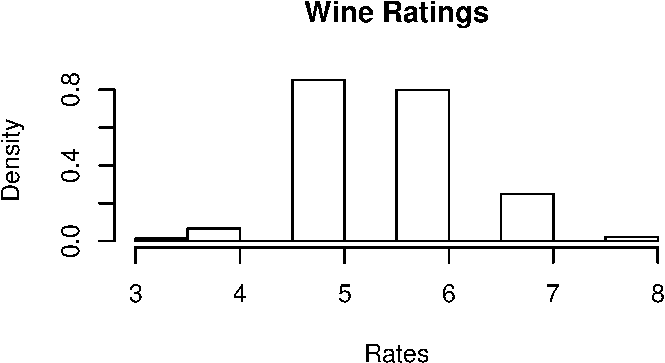
\includegraphics{./Project_files/figure-latex/unnamed-chunk-2-1.pdf}
\caption{Histogram of Quality of Wine}
\end{figure}

It's noticeable that the majority of the grades are between 5 and 6 but
it's also possible to observe that the rates are slightly skewed to 7
due the heavy tail.

The question is what is relevant for the wine to be highly rated.

To try to answer this question, it's necessary to go back to the
(cor)relation between the grades and wine characteristics described in
the data set.

\subsection{Sulfur Dioxide}\label{sulfur-dioxide}

Let's start by the Sulfur Dioxide SO\textsubscript{2}. This substance
has two main properties within the wine making process. First is to
preserve the wine, preventing from oxidation. The second is to bind the
acetaldehyde, since this last one has an unpleasant smell of bruised
apple or rank sherry and it could affect the final taste of the wine.
\cite{so2}

In the data set there are two variables dedicated to
SO\textsubscript{2}, one is called free sulfur dioxide and is a natural
result of fermentation. And the other is Total Sulfur Dioxide being the
result of the sum of free SO\textsubscript{2} and the level manually
added.

This is a good example of a pair of variable that might be correlated
and could be aggregate in a single one.

\begin{figure}[htbp]
\centering
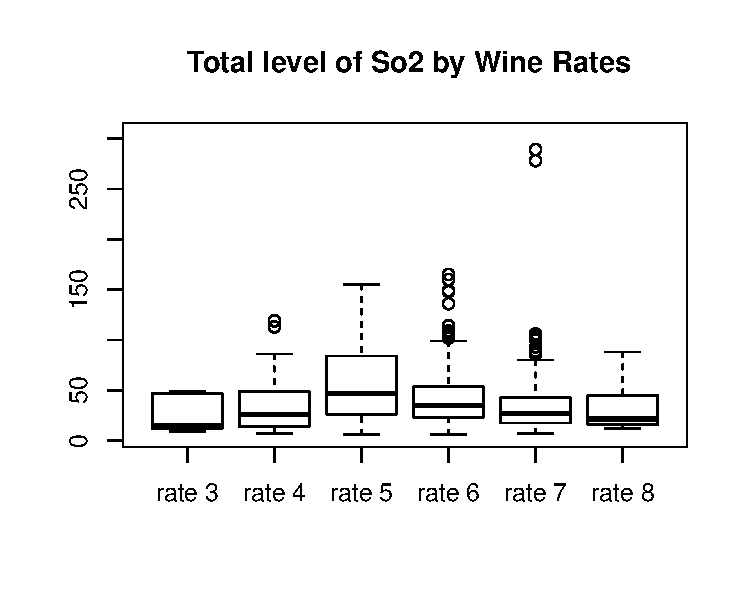
\includegraphics{./Project_files/figure-latex/unnamed-chunk-3-1.pdf}
\caption{Box plot of Level of Sulfur Dioxide by rating}
\end{figure}

\begin{longtable}[c]{@{}rrrrrr@{}}
\toprule\addlinespace
Rates & Mean & Median & Min & Max & Standard Deviation
\\\addlinespace
\midrule\endhead
3 & 15.0 & 24.90000 & 9 & 49 & 16.82888
\\\addlinespace
4 & 26.0 & 36.24528 & 7 & 119 & 27.58337
\\\addlinespace
5 & 47.0 & 56.51395 & 6 & 155 & 36.99312
\\\addlinespace
6 & 35.0 & 40.86991 & 6 & 165 & 25.03825
\\\addlinespace
7 & 27.0 & 35.02010 & 7 & 289 & 33.19121
\\\addlinespace
8 & 21.5 & 33.44444 & 12 & 88 & 25.43324
\\\addlinespace
\bottomrule
\addlinespace
\caption{Total Sulfur Dioxide Summary}
\end{longtable}

Combining the Figure 2 and the Table 1 we can see that the range level
of So\textsubscript{2} between 15 and 48 increases the likelihood of
having high rates.

\subsection{Volatile Acidity}\label{volatile-acidity}

From the correlation table it's also possible to see that Volatile
Acidity is significant for the sensorial analysis of the wine.

\begin{figure}[htbp]
\centering
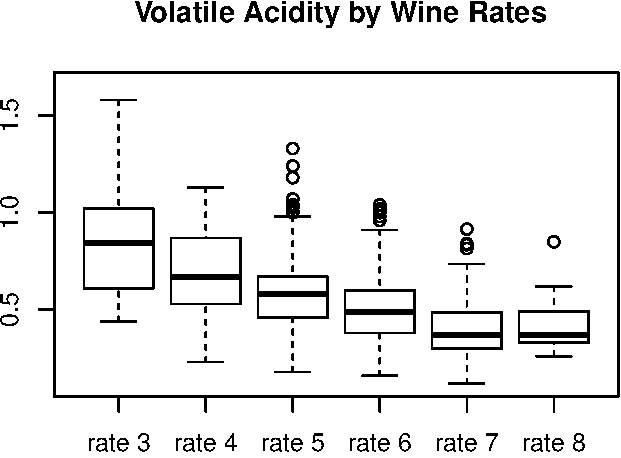
\includegraphics{./Project_files/figure-latex/unnamed-chunk-5-1.pdf}
\caption{Level of Volatile Acidity}
\end{figure}

\newpage

From Figure 2 and Table 2 it's possible to infer that the level of
alcohol has a negative correlation to the wine rates, in another words,
the lower the vol acidity the higher the rates.

\begin{longtable}[c]{@{}rrrrrr@{}}
\toprule\addlinespace
Rates & Mean & Median & Min & Max & Standard Deviation
\\\addlinespace
\midrule\endhead
3 & 0.845 & 0.8845000 & 0.44 & 1.580 & 0.3312556
\\\addlinespace
4 & 0.670 & 0.6939623 & 0.23 & 1.130 & 0.2201100
\\\addlinespace
5 & 0.580 & 0.5770411 & 0.18 & 1.330 & 0.1648012
\\\addlinespace
6 & 0.490 & 0.4974843 & 0.16 & 1.040 & 0.1609623
\\\addlinespace
7 & 0.370 & 0.4039196 & 0.12 & 0.915 & 0.1452244
\\\addlinespace
8 & 0.370 & 0.4233333 & 0.26 & 0.850 & 0.1449138
\\\addlinespace
\bottomrule
\addlinespace
\caption{Vol Acidity Summary}
\end{longtable}

\subsection{Alcohol}\label{alcohol}

From the appendix section the other relevant substance is alcohol, the
graphic and table below describe the distribution of level of alcohol
for different rates

\newpage
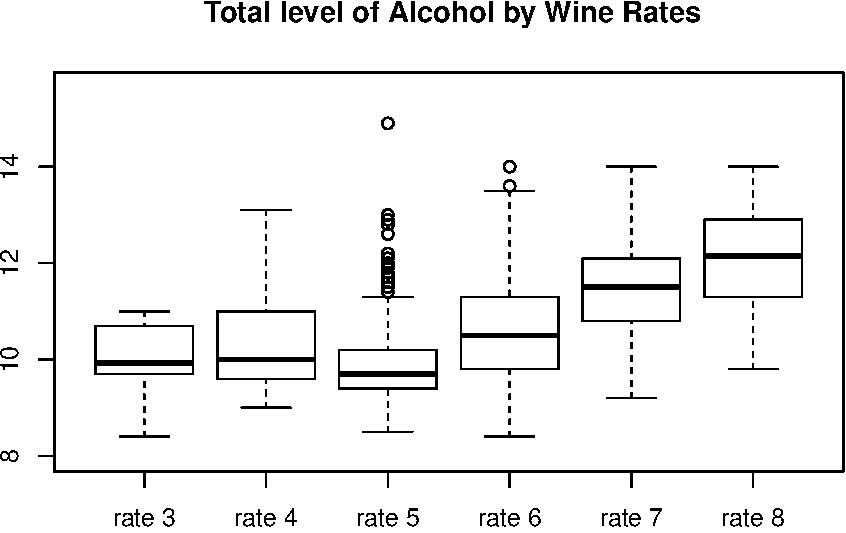
\includegraphics{./Project_files/figure-latex/unnamed-chunk-7-1.pdf}

From Figure 3 and Table 3 it's possible to infer that the level of
alcohol has a positive effect in the wine quality.

\begin{longtable}[c]{@{}rrrrrr@{}}
\toprule\addlinespace
Rates & Mean & Median & Min & Max & Standard Deviation
\\\addlinespace
\midrule\endhead
3 & 9.925 & 9.955000 & 8.4 & 11.0 & 0.8180091
\\\addlinespace
4 & 10.000 & 10.265094 & 9.0 & 13.1 & 0.9347760
\\\addlinespace
5 & 9.700 & 9.899706 & 8.5 & 14.9 & 0.7365210
\\\addlinespace
6 & 10.500 & 10.629519 & 8.4 & 14.0 & 1.0496390
\\\addlinespace
7 & 11.500 & 11.465913 & 9.2 & 14.0 & 0.9619330
\\\addlinespace
8 & 12.150 & 12.094444 & 9.8 & 14.0 & 1.2240109
\\\addlinespace
\bottomrule
\addlinespace
\caption{Alcohol Summary}
\end{longtable}

\newpage

\section{Correlation and PCA}\label{correlation-and-pca}

\subsection{Correlation Analysis}\label{correlation-analysis}

The Table 3 helps to confirm that Free SO\textsubscript{2} and Total
SO\textsubscript{2} have a significant correlation between each other.

It also confirms that the most important/relevant for high rates is
alcohol, and volatile acidity has a negative effect in the wine quality.

At this point, it's important to highlight that having a high
correlation doesn't mean having a causality.

\begin{longtable}[c]{@{}lrrrrrrrrrrrr@{}}
\toprule\addlinespace
& Acid & Vol.Acid & Citr.Acid & Sugar & Chlor & FreeSO2 & TotalSo2 & Den
& pH & Sulph & Alchool & Qlity
\\\addlinespace
\midrule\endhead
Acid & 1.00 & -0.26 & 0.67 & 0.11 & 0.09 & -0.15 & -0.11 & 0.67 & -0.68
& 0.18 & -0.06 & 0.12
\\\addlinespace
Vol.Acid & -0.26 & 1.00 & -0.55 & 0.00 & 0.06 & -0.01 & 0.08 & 0.02 &
0.23 & -0.26 & -0.20 & -0.39
\\\addlinespace
Citr.Acid & 0.67 & -0.55 & 1.00 & 0.14 & 0.20 & -0.06 & 0.04 & 0.36 &
-0.54 & 0.31 & 0.11 & 0.23
\\\addlinespace
Sugar & 0.11 & 0.00 & 0.14 & 1.00 & 0.06 & 0.19 & 0.20 & 0.36 & -0.09 &
0.01 & 0.04 & 0.01
\\\addlinespace
Chlor & 0.09 & 0.06 & 0.20 & 0.06 & 1.00 & 0.01 & 0.05 & 0.20 & -0.27 &
0.37 & -0.22 & -0.13
\\\addlinespace
FreeSO2 & -0.15 & -0.01 & -0.06 & 0.19 & 0.01 & 1.00 & 0.67 & -0.02 &
0.07 & 0.05 & -0.07 & -0.05
\\\addlinespace
TotalSo2 & -0.11 & 0.08 & 0.04 & 0.20 & 0.05 & 0.67 & 1.00 & 0.07 &
-0.07 & 0.04 & -0.21 & -0.19
\\\addlinespace
Den & 0.67 & 0.02 & 0.36 & 0.36 & 0.20 & -0.02 & 0.07 & 1.00 & -0.34 &
0.15 & -0.50 & -0.17
\\\addlinespace
pH & -0.68 & 0.23 & -0.54 & -0.09 & -0.27 & 0.07 & -0.07 & -0.34 & 1.00
& -0.20 & 0.21 & -0.06
\\\addlinespace
Sulph & 0.18 & -0.26 & 0.31 & 0.01 & 0.37 & 0.05 & 0.04 & 0.15 & -0.20 &
1.00 & 0.09 & 0.25
\\\addlinespace
Alchool & -0.06 & -0.20 & 0.11 & 0.04 & -0.22 & -0.07 & -0.21 & -0.50 &
0.21 & 0.09 & 1.00 & 0.48
\\\addlinespace
Qlity & 0.12 & -0.39 & 0.23 & 0.01 & -0.13 & -0.05 & -0.19 & -0.17 &
-0.06 & 0.25 & 0.48 & 1.00
\\\addlinespace
\bottomrule
\addlinespace
\caption{Correlation Matrix}
\end{longtable}

we can see from the table above some interesting highlights. The first
one is that we were right about the correlation between Free
SO\textsubscript{2} and Total So\textsubscript{2} variables, hence we
might combined them in one single variable.

\subsection{Principal Component
Analysis}\label{principal-component-analysis}

The application of Principal Component only depends on the data
covariance (or correlation) matrix, ie, it's not necessary to assume any
distribution for the data. Which makes the methodology much easier to
use since there's no assumption for the data distribution.\cite{pca}

The graphic below shows the main components for the explanation of the
variance. The table is built to carry the heaviest proportion of the
variance in the first components.

\begin{figure}[htbp]
\centering
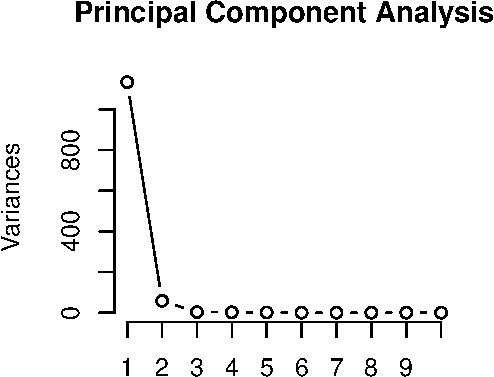
\includegraphics{./Project_files/figure-latex/unnamed-chunk-11-1.pdf}
\caption{Proportion of Variance Explained by Principal Component}
\end{figure}

\begin{longtable}[c]{@{}lll@{}}
\toprule\addlinespace
& PVE & Accumulated.PVE
\\\addlinespace
\midrule\endhead
PC1 & 94.66\% & 94.66\%
\\\addlinespace
PC2 & 4.84\% & 99.50\%
\\\addlinespace
PC3 & 0.26\% & 99.75\%
\\\addlinespace
PC4 & 0.15\% & 99.91\%
\\\addlinespace
PC5 & 0.09\% & 99.99\%
\\\addlinespace
PC6 & 0.00\% & 100.00\%
\\\addlinespace
PC7 & 0.00\% & 100.00\%
\\\addlinespace
PC8 & 0.00\% & 100.00\%
\\\addlinespace
PC9 & 0.00\% & 100.00\%
\\\addlinespace
PC10 & 0.00\% & 100.00\%
\\\addlinespace
PC11 & 0.00\% & 100.00\%
\\\addlinespace
\bottomrule
\addlinespace
\caption{Proportion of Variance Explained by Components}
\end{longtable}

The criteria to evaluate a good model is around 80 being good and
greater than 99.5 being excellent, it's important to mention that as the
variance, the PVE can variate with the problem. For this project we will
consider the first 3 component which consolidates 99.7\% of the variance
of our variables. The reason that we reduced the number of variables
from 11 to 3 is because the data set has a high correlation, therefore
it doesn't vary or it has the same variation.

Besides reducing the number of variables for the model, the component
also highlights any particular evidence for clusters.

\begin{longtable}[c]{@{}lll@{}}
\toprule\addlinespace
& Variables & EigenValues
\\\addlinespace
\midrule\endhead
11 & Alcohol & 0
\\\addlinespace
10 & Sulphates & 0.04
\\\addlinespace
9 & PH & 0.1
\\\addlinespace
8 & Density & 0.11
\\\addlinespace
7 & Total Sulfur Dioxide & 0.15
\\\addlinespace
6 & Free Sulfur Dioxide & 0.2
\\\addlinespace
5 & Chlorides & 1.02
\\\addlinespace
4 & Residual Sugar & 1.35
\\\addlinespace
3 & Citric Acid & 1.76
\\\addlinespace
1 & Fixed Acidity & 33.67
\\\addlinespace
2 & Volatile Acidity & 7.61
\\\addlinespace
\bottomrule
\addlinespace
\caption{Eigenvalues}
\end{longtable}

Based on eigenvalues we can observe that Acidity is more mixed within
the rates in a way that most of the variability of the model are in
these two variables.

Alcohol, Sulfate and Density for example are substances that are
important to the final grade, since their variability is very important
and they have a positive correlation to the increase of the rates.

Plotting the first two components we have the following graph:

\begin{verbatim}
## Loading required package: grid
## Loading required package: quadprog
\end{verbatim}

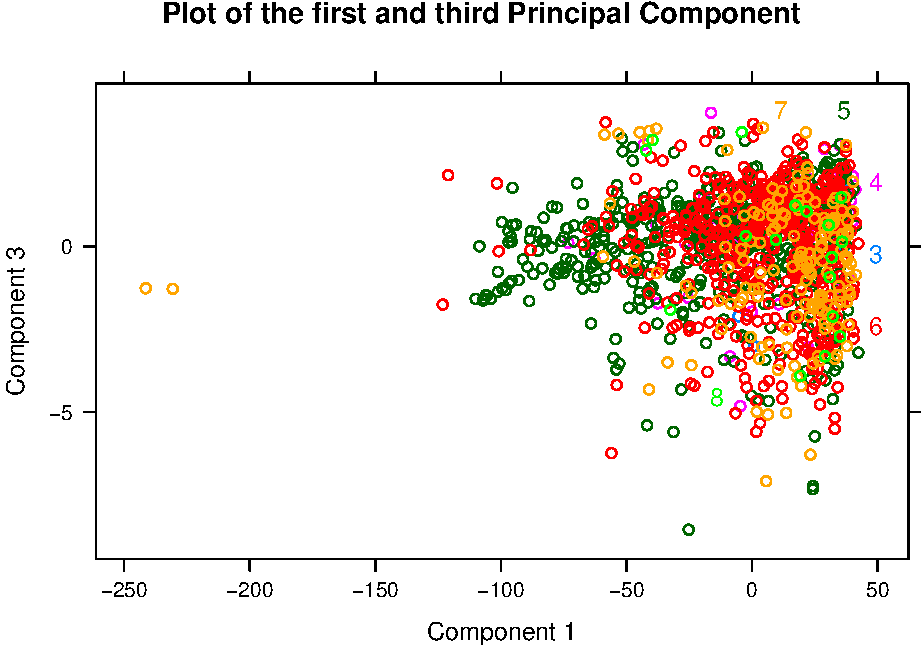
\includegraphics{./Project_files/figure-latex/unnamed-chunk-14-1.pdf} We
can see that the 5 rates is lower but also more expanded than the
others.

\newpage

\section{Classification Model}\label{classification-model}

The classification methodology that we'll be using in this document is
the Logistic Regression. The reason we chose this model rather than the
other classification methodologies is because this method shares the
properties of all other memory-based classification methods - defer most
of the processing of the training data point until after a query is made
- and has some particular qualities like simplicity, capability of
extrapolating and a known confidence interval. \cite{log}

\begin{verbatim}
## 
## Call:
## glm(formula = formula_raw, family = binomial(), data = data_2)
## 
## Deviance Residuals: 
##      Min        1Q    Median        3Q       Max  
## -2.96787   0.00752   0.02341   0.05730   1.22446  
## 
## Coefficients:
##                        Estimate Std. Error z value Pr(>|z|)    
## (Intercept)           494.89510  523.99352   0.944 0.344931    
## fixed.acidity          -0.28791    0.67009  -0.430 0.667446    
## volatile.acidity       -8.40765    2.50988  -3.350 0.000809 ***
## citric.acid            -3.70698    3.92708  -0.944 0.345195    
## residual.sugar          0.14205    0.29387   0.483 0.628827    
## chlorides             -13.03262    7.00680  -1.860 0.062886 .  
## free.sulfur.dioxide    -0.15367    0.08888  -1.729 0.083823 .  
## total.sulfur.dioxide    0.09925    0.04981   1.992 0.046322 *  
## density              -470.45027  533.58716  -0.882 0.377953    
## pH                     -8.01302    4.80305  -1.668 0.095253 .  
## sulphates               2.69403    3.47425   0.775 0.438088    
## alcohol                 1.32310    0.77934   1.698 0.089563 .  
## ---
## Signif. codes:  0 '***' 0.001 '**' 0.01 '*' 0.05 '.' 0.1 ' ' 1
## 
## (Dispersion parameter for binomial family taken to be 1)
## 
##     Null deviance: 121.428  on 1598  degrees of freedom
## Residual deviance:  69.165  on 1587  degrees of freedom
## AIC: 93.165
## 
## Number of Fisher Scoring iterations: 10
\end{verbatim}

The table above shows the scores for all variables. Based on the last
column, it's possible to choose the relevant coefficients (with p-value
\textless{} 0.10). So for the final model we have:

\begin{itemize}

\item volatility acidity;
\item chlorides;
\item free sulfur dioxide;
\item pH;
\item alcohol
 \end{itemize}

Alcohol is the only compound that as higher the level the better. All
the others affect the wine flavor/quality negatively. This way it's
possible to predict the rate based on the coefficients above.

Now applying the same methodology to the PCA data set we have the
following output:

\begin{verbatim}
## 
## Call:
## glm(formula = formula, family = binomial(), data = data_pca)
## 
## Deviance Residuals: 
##     Min       1Q   Median       3Q      Max  
## -3.4683   0.0580   0.1033   0.1417   0.1990  
## 
## Coefficients:
##             Estimate Std. Error z value Pr(>|z|)    
## (Intercept)  5.76102    0.64052   8.994   <2e-16 ***
## comp1       -0.04768    0.02530  -1.885   0.0594 .  
## comp2       -0.05441    0.07312  -0.744   0.4568    
## comp3        0.01174    0.17916   0.066   0.9477    
## ---
## Signif. codes:  0 '***' 0.001 '**' 0.01 '*' 0.05 '.' 0.1 ' ' 1
## 
## (Dispersion parameter for binomial family taken to be 1)
## 
##     Null deviance: 121.43  on 1598  degrees of freedom
## Residual deviance: 114.29  on 1595  degrees of freedom
## AIC: 122.29
## 
## Number of Fisher Scoring iterations: 9
\end{verbatim}

So Based on the table above only the the first component is relevant for
the model, and as higher the value, the worse is the rating.

The only problem of having the pca model is the machine learning cost,
because the algorithm would have to run the PCA and then using this
``new data'' we would have the logistic model. When we are dealing with
huge data sets this becomes expansive.

\subsection{Machine Learning - 10 Cross Folder
Validation}\label{machine-learning---10-cross-folder-validation}

Now we need to run the cross validation for 10 folders. Based on the
data below we can see that our model is very accurate. We have one loop
with 3 prediction error over 67\%

But still very accurate.

\begin{verbatim}
## Loading required package: ggplot2
\end{verbatim}

\begin{verbatim}
## [1] "Prediction Table for validation 1"
## 
##    0 0.14 0.17  0.2 0.25 0.33  0.4  0.5 
##  101   14   22   14    5    1    1    1 
## [1] "Confusion Matrix for validation 1"
##    
##      3  4  5  6  7  8
##   3  0  0  0  0  0  0
##   4  1  0  0  0  0  0
##   5  0  3 54 21  0  0
##   6  0  1 14 41 14  2
##   7  0  0  1  1  6  0
##   8  0  0  0  0  0  0
## [1] "Prediction Table for validation 2"
## 
##    0 0.14 0.17  0.2 0.25  0.5 
##   98   17   17   20    5    4 
## [1] "Confusion Matrix for validation 2"
##    
##      4  5  6  7  8
##   3  0  0  0  0  0
##   4  0  0  0  0  0
##   5  4 47 15  0  0
##   6  4 20 47 17  1
##   7  0  0  2  4  0
##   8  0  0  0  0  0
## [1] "Prediction Table for validation 3"
## 
##    0 0.12 0.14 0.17  0.2 0.25 0.29    1 
##  104    1   13   19   15    4    2    1 
## [1] "Confusion Matrix for validation 3"
##    
##      3  4  5  6  7  8
##   3  0  0  0  0  0  0
##   4  0  0  0  0  0  0
##   5  0  3 55 14  2  0
##   6  1  0 15 45 13  1
##   7  0  0  0  5  4  1
##   8  0  0  0  0  0  0
## [1] "Prediction Table for validation 4"
## 
##    0 0.12 0.14 0.17  0.2 0.25  0.4  0.5 
##   91    1   16   19   24    6    1    1 
## [1] "Confusion Matrix for validation 4"
##    
##      4  5  6  7  8
##   3  0  0  0  0  0
##   4  0  1  0  0  0
##   5  5 43 16  0  0
##   6  1 23 45 16  1
##   7  0  1  3  3  1
##   8  0  0  0  0  0
## [1] "Prediction Table for validation 5"
## 
##    0 0.12 0.14 0.17  0.2 0.25  0.5 
##   95    1   12   25   24    2    2 
## [1] "Confusion Matrix for validation 5"
##    
##      4  5  6  7  8
##   3  0  0  0  0  0
##   4  0  1  0  0  0
##   5  2 47 23  0  0
##   6  2 23 39 12  0
##   7  0  0  2  9  1
##   8  0  0  0  0  0
## [1] "Prediction Table for validation 6"
## 
##    0 0.12 0.14 0.17  0.2 0.25 0.29  0.4  0.5  0.6 
##   87    1   10   30   23    4    2    1    1    1 
## [1] "Confusion Matrix for validation 6"
##    
##      4  5  6  7  8
##   3  0  0  0  0  0
##   4  0  0  0  0  0
##   5  2 46 24  2  0
##   6  1 23 34 10  2
##   7  0  1  6  7  1
##   8  0  1  0  0  0
## [1] "Prediction Table for validation 7"
## 
##    0 0.12 0.14 0.17  0.2 0.25  0.5 0.67 
##   96    1   19   19   16    7    1    2 
## [1] "Confusion Matrix for validation 7"
##    
##      3  4  5  6  7  8
##   3  0  0  0  0  0  0
##   4  0  1  0  0  0  0
##   5  2  6 49 18  0  0
##   6  0  1 16 45 19  1
##   7  0  0  0  1  1  1
##   8  0  0  0  0  0  0
## [1] "Prediction Table for validation 8"
## 
##    0 0.12 0.14 0.17  0.2 0.25 0.29  0.5 0.67 
##   94    1   16   23   18    5    1    1    1 
## [1] "Confusion Matrix for validation 8"
##    
##      3  4  5  6  7  8
##   3  0  0  0  0  0  0
##   4  0  0  0  0  0  0
##   5  1  5 49 19  1  0
##   6  0  1 18 41 16  0
##   7  0  0  0  4  4  1
##   8  0  0  0  0  0  0
## [1] "Prediction Table for validation 9"
## 
##    0 0.12 0.14 0.17  0.2 0.25 0.29  0.5 0.67 
##   93    1   14   18   24    3    1    4    3 
## [1] "Confusion Matrix for validation 9"
##    
##      3  4  5  6  7  8
##   3  0  0  0  0  0  0
##   4  0  0  0  0  0  0
##   5  3  1 43 15  1  0
##   6  0  4 24 46 14  2
##   7  0  0  0  3  4  1
##   8  0  0  0  0  0  0
## [1] "Prediction Table for validation 10"
## 
##    0 0.14 0.17  0.2 0.25 0.29  0.5 0.67 
##   93   19   18   18    4    1    3    2 
## [1] "Confusion Matrix for validation 10"
##    
##      3  4  5  6  7  8
##   3  0  0  0  0  0  0
##   4  0  0  1  0  0  0
##   5  2  3 48 18  1  0
##   6  0  3 17 45 19  1
##   7  0  0  0  0  0  0
##   8  0  0  0  0  0  0
\end{verbatim}

\section{Comparison to other models}\label{comparison-to-other-models}

One of the final goals of this project is to compare with other models,
in this case.

Comparing the methodology and the results in this document to the
reference it's possible to see very similar results considering 90\%
accuracy since the methodology is the same. These are the main
similarities and discrepancies from the model proposed here and the
author methodology:

\begin{itemize}

\item in the reference the authors apply different fitting criteria in order to consider the data well fitted (p. 25). In this project it's showed only one criteria which is 90% accuracy. Maybe if it was considered another criteria we'd have a different conclusion.
\item the authors applied 20 runs of a 5 cross folder validation, while in this project we have only 1 run for 10 cross folder validation. This could be affect the results since it's not as confused as it should be.
\item the authors ignored grades 3 and 9 since they were very rare within the data set. This was a very good approached since the rates 9 and 3 hurt the model results being to hard to predict.

 \end{itemize}

\section{Conclusion}\label{conclusion}

Based on the methodology applied above we can infer that the relevant
compounds to predict the wine rates are:

\begin{itemize}

\item volatility acidity having a negative effect;
\item chlorides having a negative effect;
\item free sulfur dioxide having a negative effect;
\item pH having a negative effect;
\item alcohol having a positive effect
 \end{itemize}

The Logistic Model predicts with an error lower than 25\% 95\% of the
times that we ran the algorithm.

The rate is most common to be misplaced is 5 because the variability of
the compounds is too high to have a distinct group.

The computational cost for the algorithm is relatively low making
possible the automation and deployment into a quality assurance process.

\section{References}\label{references}

\begin{thebibliography}{1}
\bibitem{so2} Gawel Richard (Uknown period). Retrieved from \url{http://www.aromadictionary.com/articles/sulfurdioxide_article.html}

\bibitem{pca} Johnson and Wichern. (pag. 459 - 462) Retrieved from {\em Applied Multivariate Statistical Analysis}

\bibitem{log}Deng Kan. (1999. April 09) Retrieved from \url{https://www.cs.cmu.edu/~kdeng/thesis/logistic.pdf}

\bibitem{volacit}Pandell J Alexander. (1999) Retrieved from \url{http://www.wineperspective.com/the_acidity_of_wine.htm}

\bibitem{comp} Paulo Cortez, Antonio Cerdeira and Fernando Almeida. (Unknown) Retrieved from \url{http://repositorium.sdum.uminho.pt/bitstream/1822/10029/1/wine5.pdf}

\end{thebibliography}

\section{Appendix}\label{appendix}

Histogram of all Variables

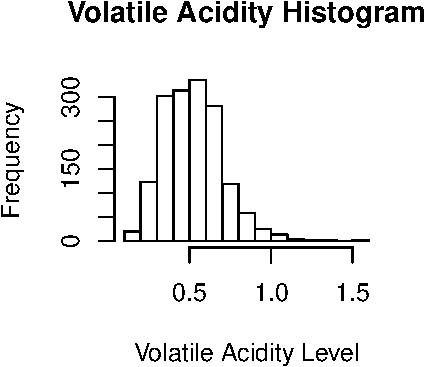
\includegraphics{./Project_files/figure-latex/unnamed-chunk-18-1.pdf}
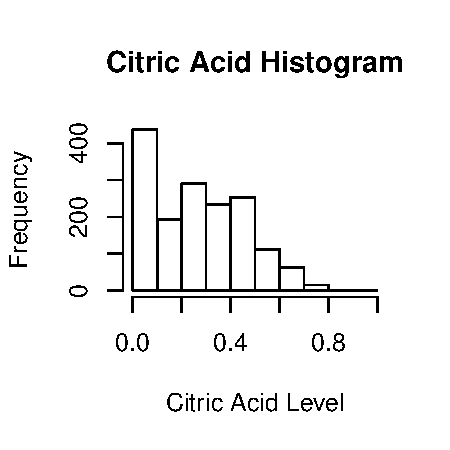
\includegraphics{./Project_files/figure-latex/unnamed-chunk-18-2.pdf}
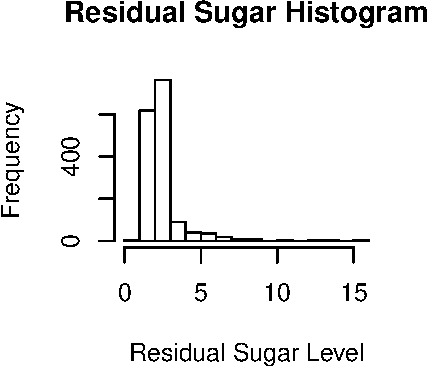
\includegraphics{./Project_files/figure-latex/unnamed-chunk-18-3.pdf}
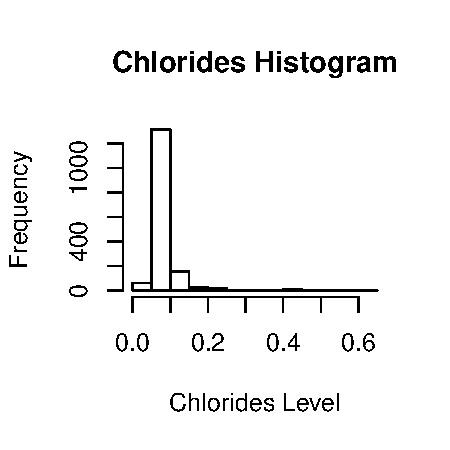
\includegraphics{./Project_files/figure-latex/unnamed-chunk-18-4.pdf}
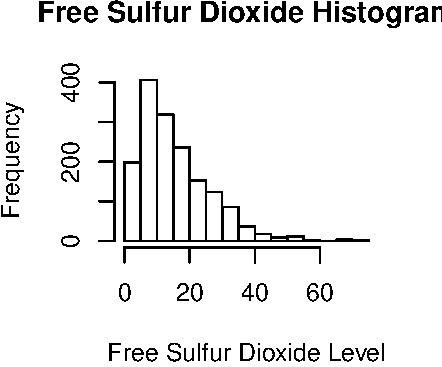
\includegraphics{./Project_files/figure-latex/unnamed-chunk-18-5.pdf}
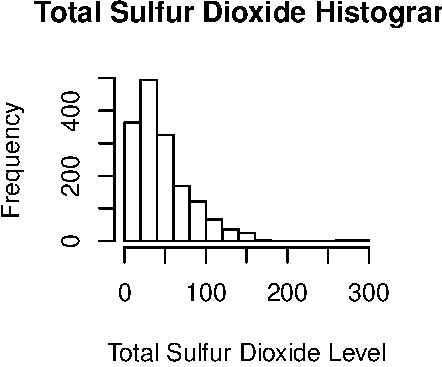
\includegraphics{./Project_files/figure-latex/unnamed-chunk-18-6.pdf}
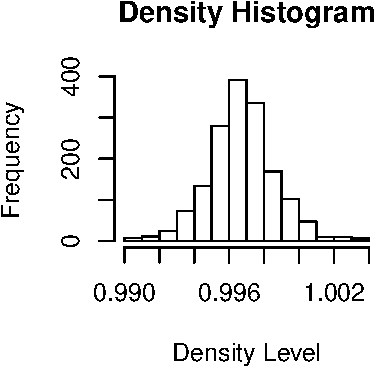
\includegraphics{./Project_files/figure-latex/unnamed-chunk-18-7.pdf}
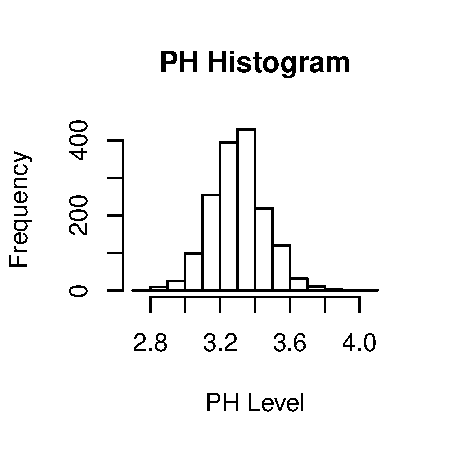
\includegraphics{./Project_files/figure-latex/unnamed-chunk-18-8.pdf}
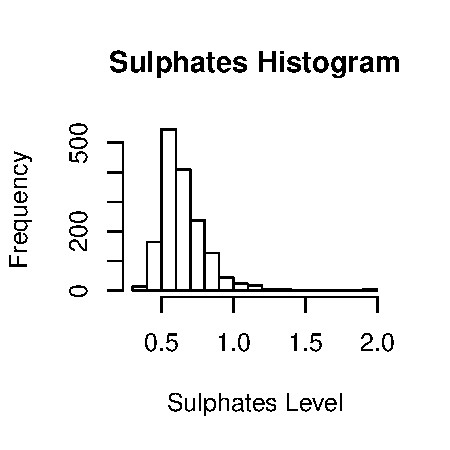
\includegraphics{./Project_files/figure-latex/unnamed-chunk-18-9.pdf}
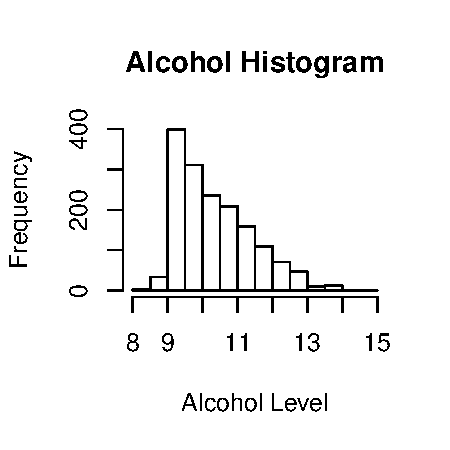
\includegraphics{./Project_files/figure-latex/unnamed-chunk-18-10.pdf}
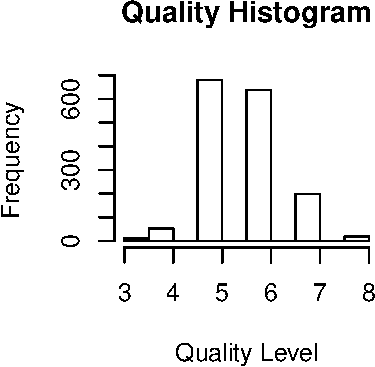
\includegraphics{./Project_files/figure-latex/unnamed-chunk-18-11.pdf}

\end{document}
